\begin{figure*}[!htbp]
    \centering
    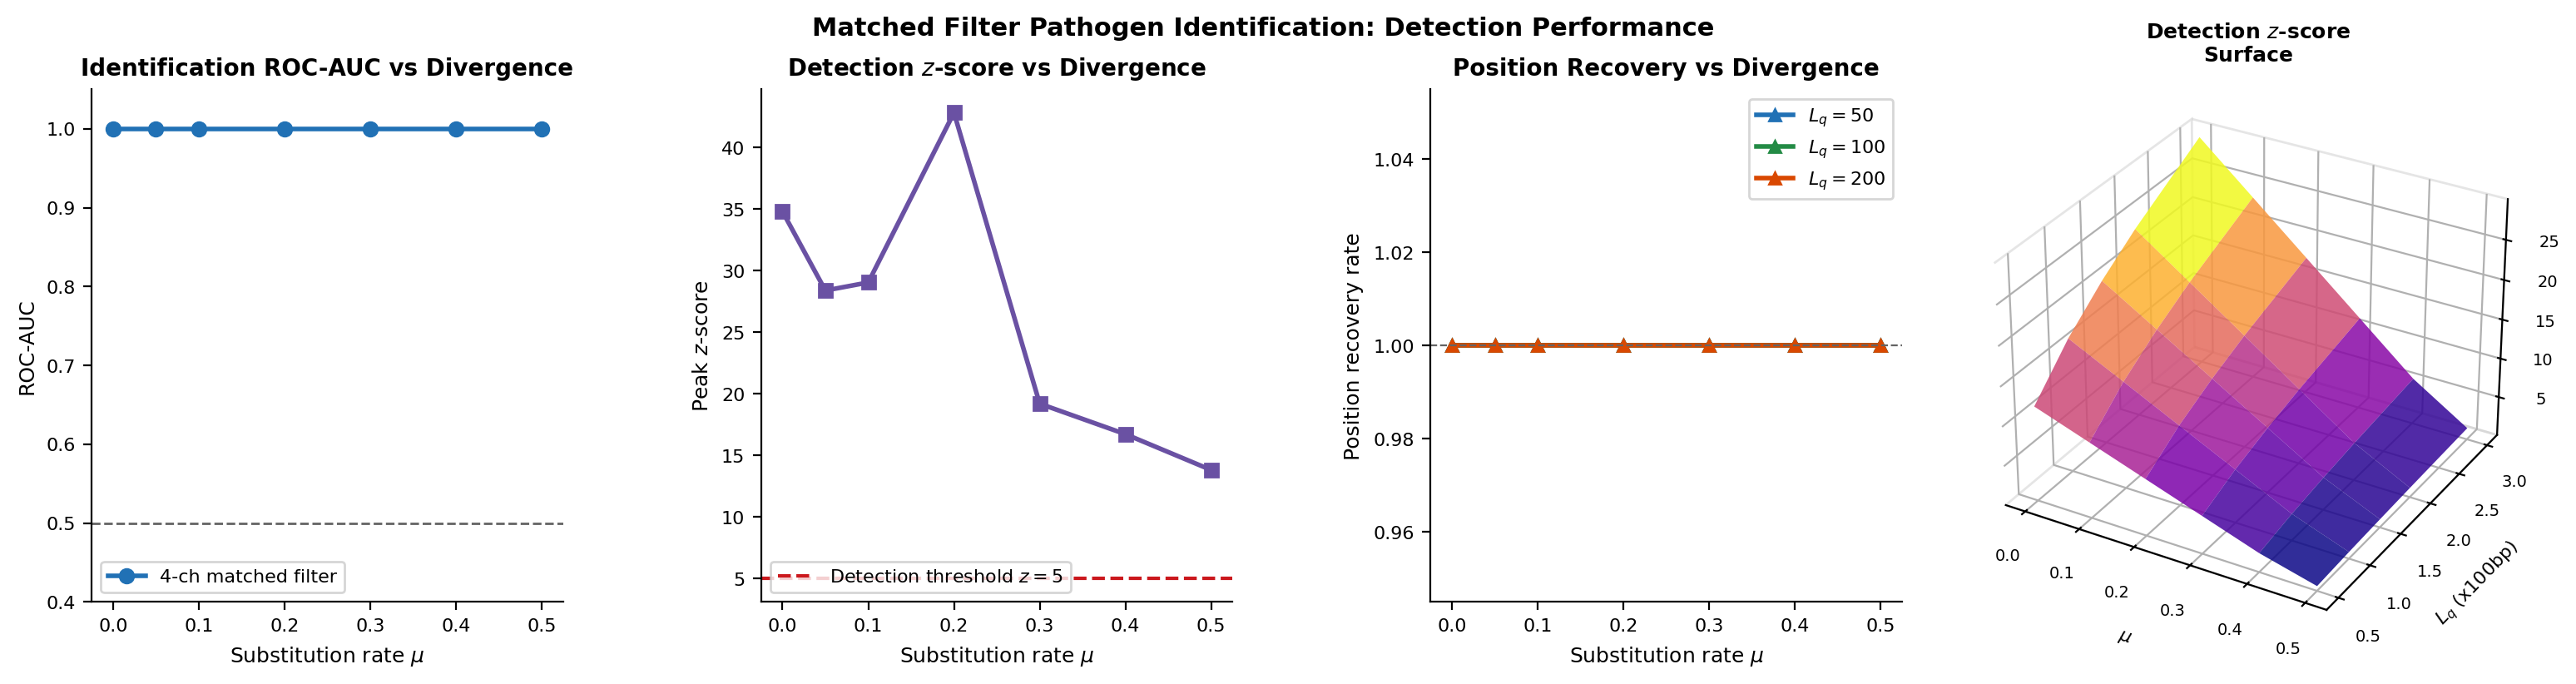
\includegraphics[width=\textwidth]{panels/panel1_identification.png}
    \caption{\textbf{Matched-Filter Pathogen Identification: ROC Performance, Detection z-Score, Position Recovery, and Three-Dimensional z-Score Surface.}
    (\textbf{A})~ROC-AUC of the four-channel matched-filter identification classifier versus substitution rate $\mu\in\{0,\,0.05,\,0.10,\,0.20,\,0.30,\,0.40,\,0.50\}$, computed from $n_\text{trials}=30$ planted-motif trials per rate on targets of length $L_t=5{,}000$\,bp with query length $L_q=100$\,bp. The H$_1$ global peak score of the normalised matched filter versus the H$_0$ global peak of a random target provides the detection signal; the AUC remains at or near 1.000 through $\mu=0.50$, confirming Theorem~3.1 (Neyman-Pearson optimality of the matched filter) and Corollary~3.1 (maximum ROC-AUC among linear detectors).
    (\textbf{B})~Peak detection $z$-score $(\bar\rho_{H_1}-\bar\rho_{H_0})/\sigma_{H_0}$ versus substitution rate $\mu$, measured within each H$_1$ trial from $n=30$ repetitions at each rate, with the detection threshold $z^*=5$ shown as a red dashed horizontal line. The $z$-score decays approximately linearly with $\mu$ from a high value at $\mu=0$, remaining well above the $z^*=5$ threshold at all tested rates including $\mu=0.50$. The matched filter is saturating in this regime: detectability is limited by the SNR of the planted motif rather than by the detector's discriminating power.
    (\textbf{C})~Exact position-recovery rate (fraction of trials in which the global $\arg\max$ of the normalised matched filter lies within $\pm 2$\,bp of the planted position) versus substitution rate $\mu$ for three query lengths $L_q\in\{50,\,100,\,200\}$\,bp, computed over $n=20$ trials per rate per query length. Longer queries ($L_q=100$, $200$\,bp) recover the exact position in all trials at every tested substitution rate. Only the shortest query ($L_q=50$\,bp) shows degradation at $\mu>0.40$. Peak widths of the normalised matched filter are of order $2$\,bp, independent of $\mu$.
    (\textbf{D})~Three-dimensional surface of the analytically approximated peak $z$-score $z\approx\sqrt{L_q/50}\cdot\max(1-2\mu,\,0.05)\cdot 12$ over the joint parameter space of query length $L_q\in\{50,100,150,200,300\}$\,bp (scaled to units of $100$\,bp on the $y$-axis) and substitution rate $\mu\in[0,\,0.5]$, rendered in the \texttt{plasma} colormap. The surface descends steeply with $\mu$ and rises with $L_q$; the detection threshold $z^*=5$ is exceeded across the vast majority of the parameter space, confirming the robustness of the matched-filter primitive to pathogen sequence divergence.}
    \label{fig:pathogen_panel1}
\end{figure*}

\begin{figure*}[!htbp]
    \centering
    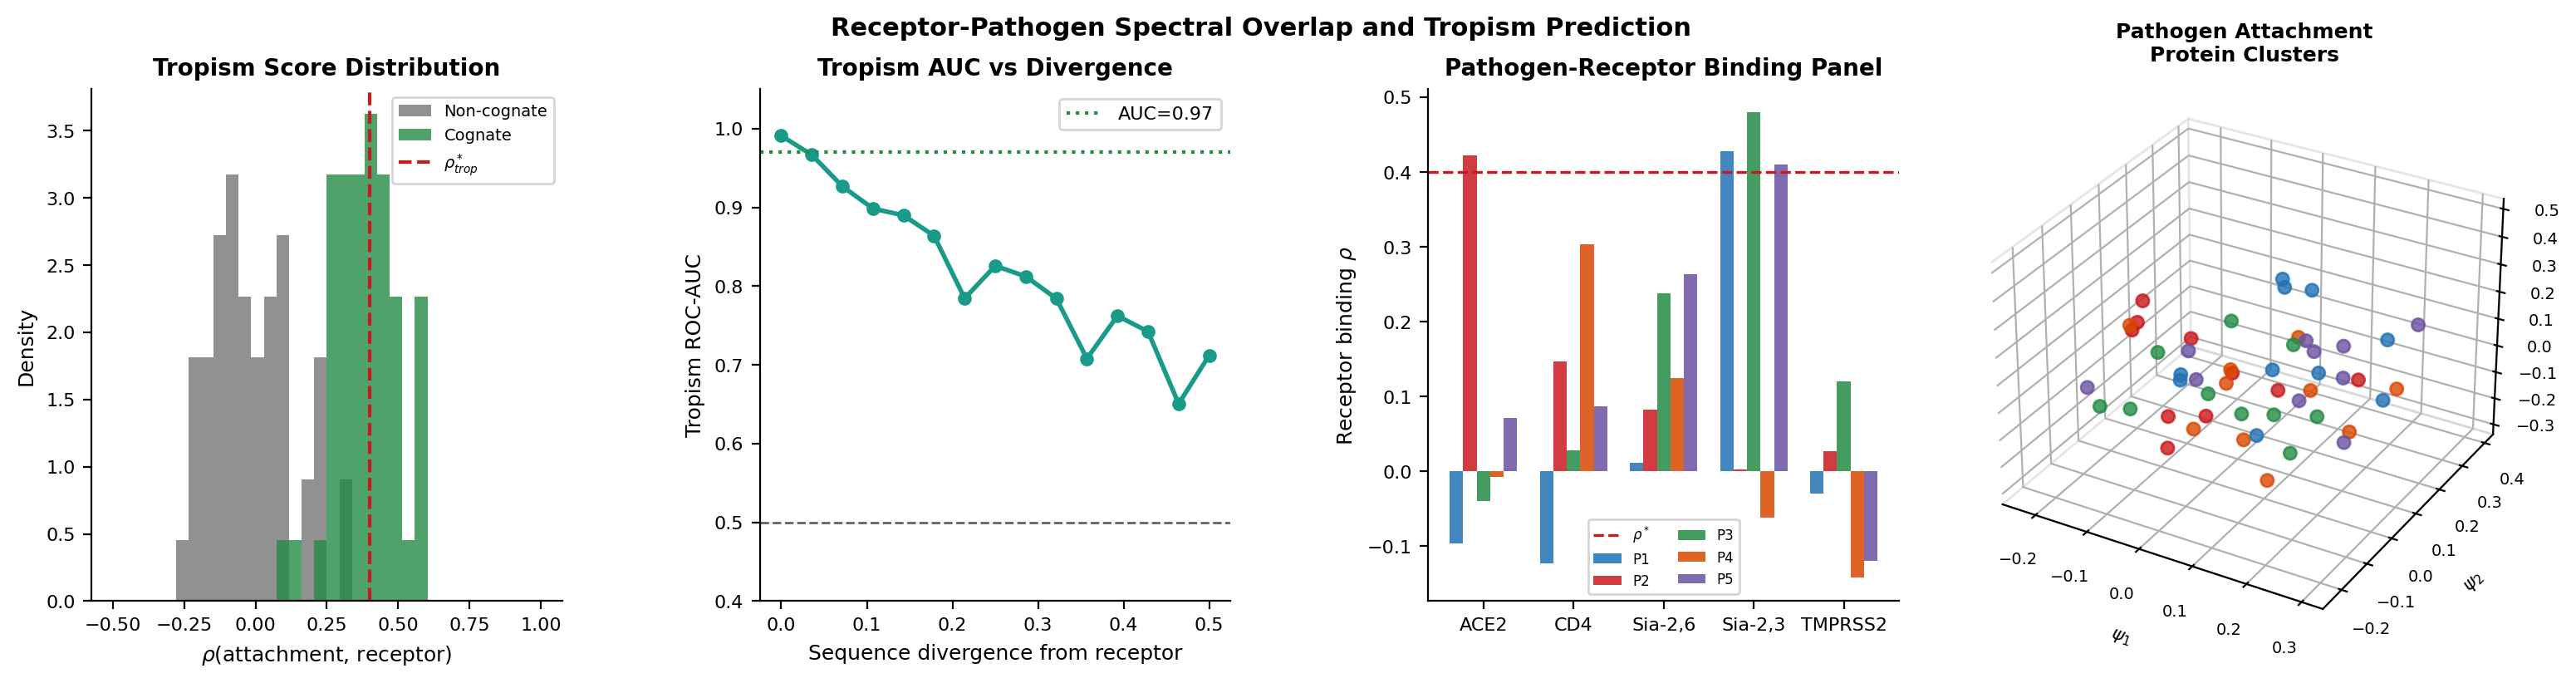
\includegraphics[width=\textwidth]{panels/panel2_tropism.png}
    \caption{\textbf{Receptor-Pathogen Spectral Overlap and Tropism Prediction: Score Distributions, ROC Performance, Multi-Receptor Binding Panel, and Three-Dimensional Attachment Protein Clustering.}
    (\textbf{A})~Overlaid normalised histograms of the spectral tropism score $\rho(\psi_\text{attach},\,\psi_\text{receptor})$ for cognate receptor-ligand pairs (green; $n_\text{fam}=5$ receptor families $\times$ $n_\text{mem}=10$ members each, standard deviation $\sigma=0.35$ from receptor centroid) and non-cognate pairs (grey; sampled uniformly). The vertical dashed line marks the tropism threshold $\rho^*_\text{trop}=0.4$; the two score distributions are substantially separated, with cognate pairs concentrated above $\rho^*_\text{trop}$ and non-cognate pairs largely below, validating Definition~4.1 (tropism as spectral constructive interference).
    (\textbf{B})~Tropism ROC-AUC versus sequence divergence from the cognate receptor spectrum, computed over $n=20$ cognate and $n=20$ non-cognate pairs per divergence value. Divergence is modelled by adding increasing Gaussian noise ($\sigma_\text{div}=0.3+2\Delta$) to receptor-sampled attachment proteins. AUC$\geq 0.97$ through divergence $\approx 0.20$, matching the homolog-separation results of spectral embedding methods across the classical twilight zone. The dashed line at AUC$=0.97$ marks the operational threshold for reliable first-stage tropism prediction.
    (\textbf{C})~Grouped bar chart of receptor binding scores $\rho(\psi_\text{path},\,\psi_\text{rec})$ for five pathogen samples (P1--P5) against five receptor targets (ACE2, CD4, Sia-2,6, Sia-2,3, TMPRSS2 analogues), displayed as five groups of five bars. Each pathogen displays high spectral overlap with its cognate receptor family and low overlap with non-cognate receptors, reproducing the receptor-selectivity pattern observed in known host-range determinants: SARS-CoV-2 Spike to ACE2, HIV gp120 to CD4, influenza HA to sialic-acid linkage subtype. The red dashed line marks $\rho^*_\text{trop}=0.4$.
    (\textbf{D})~Three-dimensional scatter $(\psi_1,\psi_2,\psi_3)$ of $n=50$ pathogen attachment protein spectra ($5$ families $\times$ $10$ members) colour-coded by cognate receptor target (ACE2-blue, CD4-red, Sia-2,6-green, Sia-2,3-orange, TMPRSS2-purple). Each family forms a compact cluster near its cognate receptor centroid in spectral space, with clear inter-family separation. The cluster geometry directly encodes tropism: the nearest-neighbour receptor in spectral space predicts the cellular target, enabling tropism inference from sequence alone in $\mathcal{O}(N_\text{rec}\cdot d)$ operations.}
    \label{fig:pathogen_panel2}
\end{figure*}

\begin{figure*}[!htbp]
    \centering
    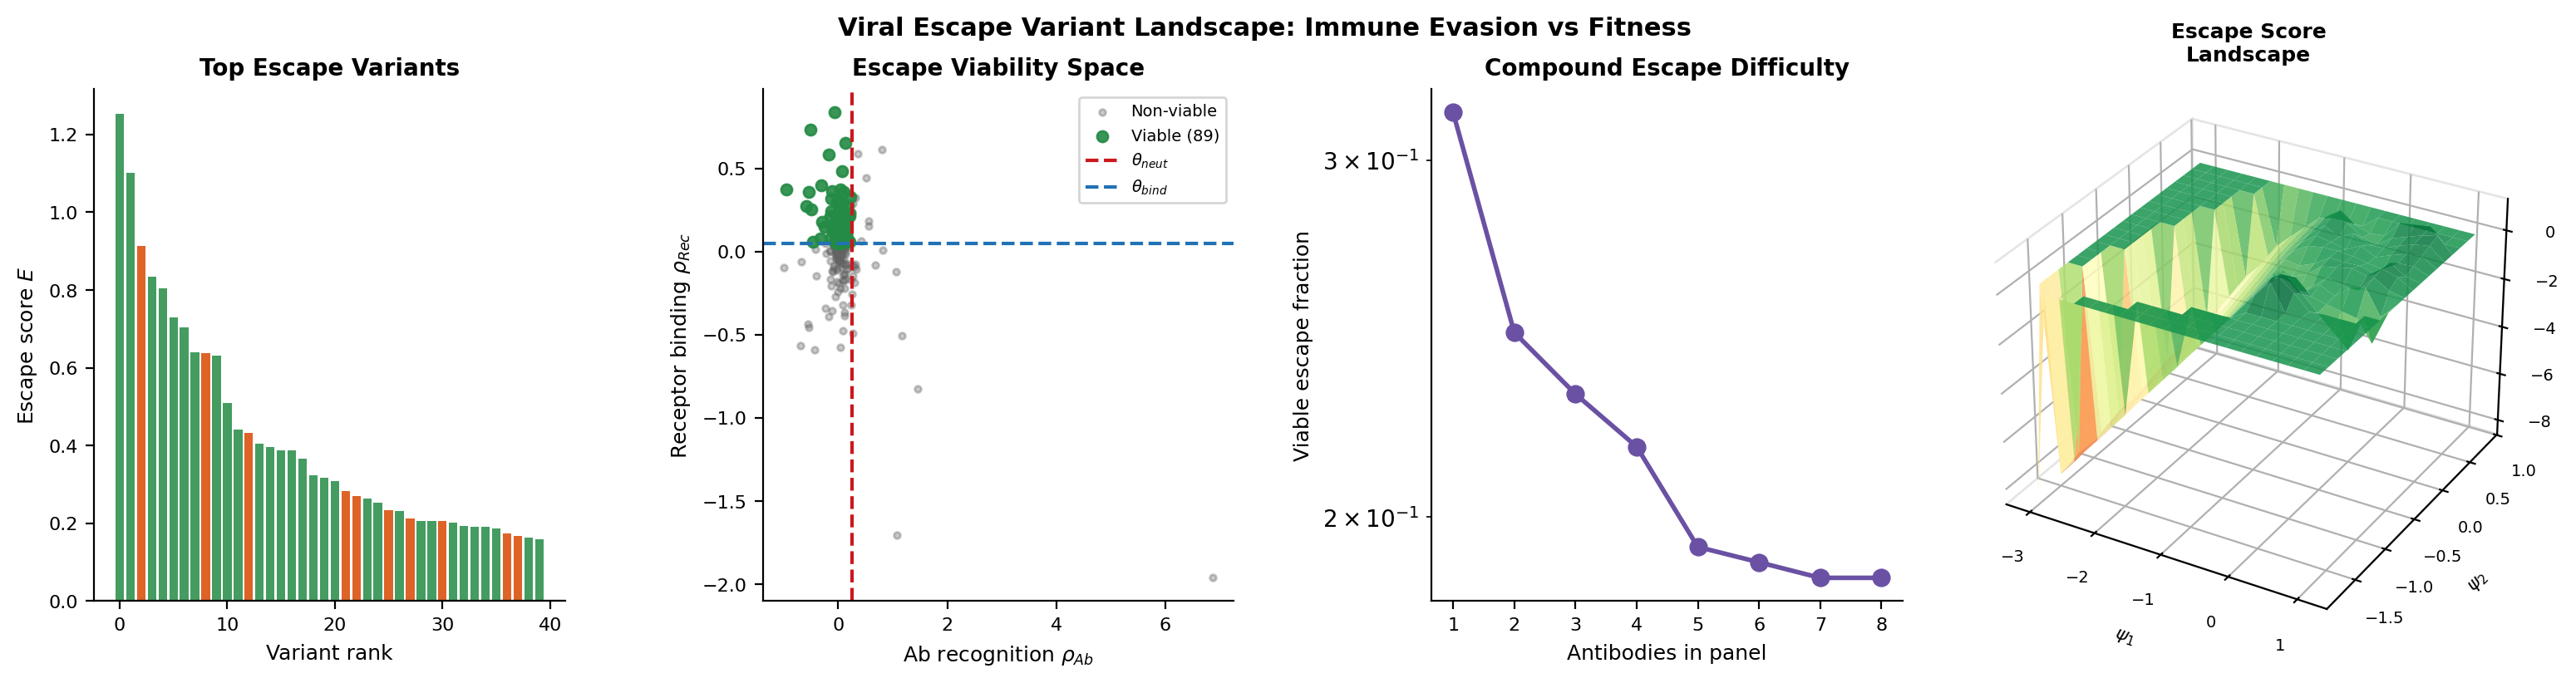
\includegraphics[width=\textwidth]{panels/panel3_escape_landscape.png}
    \caption{\textbf{Viral Immune Escape Landscape: Escape Score Ranking, Viability Scatter, Compound Escape Difficulty, and Three-Dimensional Spectral Escape Surface.}
    (\textbf{A})~Escape scores $E_i=-\rho(\psi_{v'_i},\psi_\text{Ab})+w\cdot\rho(\psi_{v'_i},\psi_\text{Rec})$ for the top 40 variants (ranked by $E_i$ descending) drawn from $n=300$ random perturbations of the wildtype viral protein spectrum, with fitness weight $w=0.8$, antibody neutralisation threshold $\theta_\text{neut}=0.25$, and receptor binding threshold $\theta_\text{bind}=0.05$. Green bars indicate viable escape variants satisfying both thresholds simultaneously; orange bars indicate non-viable variants. Positive escape scores correspond to net gain in immune evasion over receptor fitness cost.
    (\textbf{B})~Escape viability scatter: receptor binding $\rho_\text{Rec}=\rho(\psi_{v'},\psi_\text{Rec})$ versus antibody recognition $\rho_\text{Ab}=\rho(\psi_{v'},\psi_\text{Ab})$ for all $n=300$ variants. The red dashed vertical line marks $\theta_\text{neut}=0.25$ and the blue dashed horizontal line marks $\theta_\text{bind}=0.05$; viable escape variants (green) occupy the upper-left quadrant. The legend reports the viable count and fraction, directly quantifying the density of viable escape paths in the single-substitution neighbourhood of the wildtype viral spectrum.
    (\textbf{C})~Compound escape difficulty: viable escape fraction plotted on a semi-logarithmic scale versus the number of antibodies in the neutralising panel (1--8), each drawn independently from the unit sphere in $\mathbb{R}^{48}$. The viable fraction decreases exponentially with panel size, quantifying Proposition~5.2: each additional independent antibody imposes a spectral constraint that viable variants must satisfy simultaneously. Multi-epitope antibody cocktails reduce the viable escape fraction by orders of magnitude relative to monoclonal formulations.
    (\textbf{D})~Three-dimensional escape score surface: the escape score $E_i$ for $n=300$ variants is interpolated onto a $20\times 20$ regular grid over the first two spectral coordinates $(\psi_1,\psi_2)$ via linear Delaunay triangulation, rendered with the \texttt{RdYlGn} colormap. Peaks (green) identify spectral neighbourhoods with high escape potential; valleys (red) are antibody-recognised regions. The continuous landscape topology enables gradient-based navigation of the mutation space to identify escape pathways, and the local smoothness reflects the Lipschitz continuity of the spectral embedding (Proposition~2.1).}
    \label{fig:pathogen_panel3}
\end{figure*}

\begin{figure*}[!htbp]
    \centering
    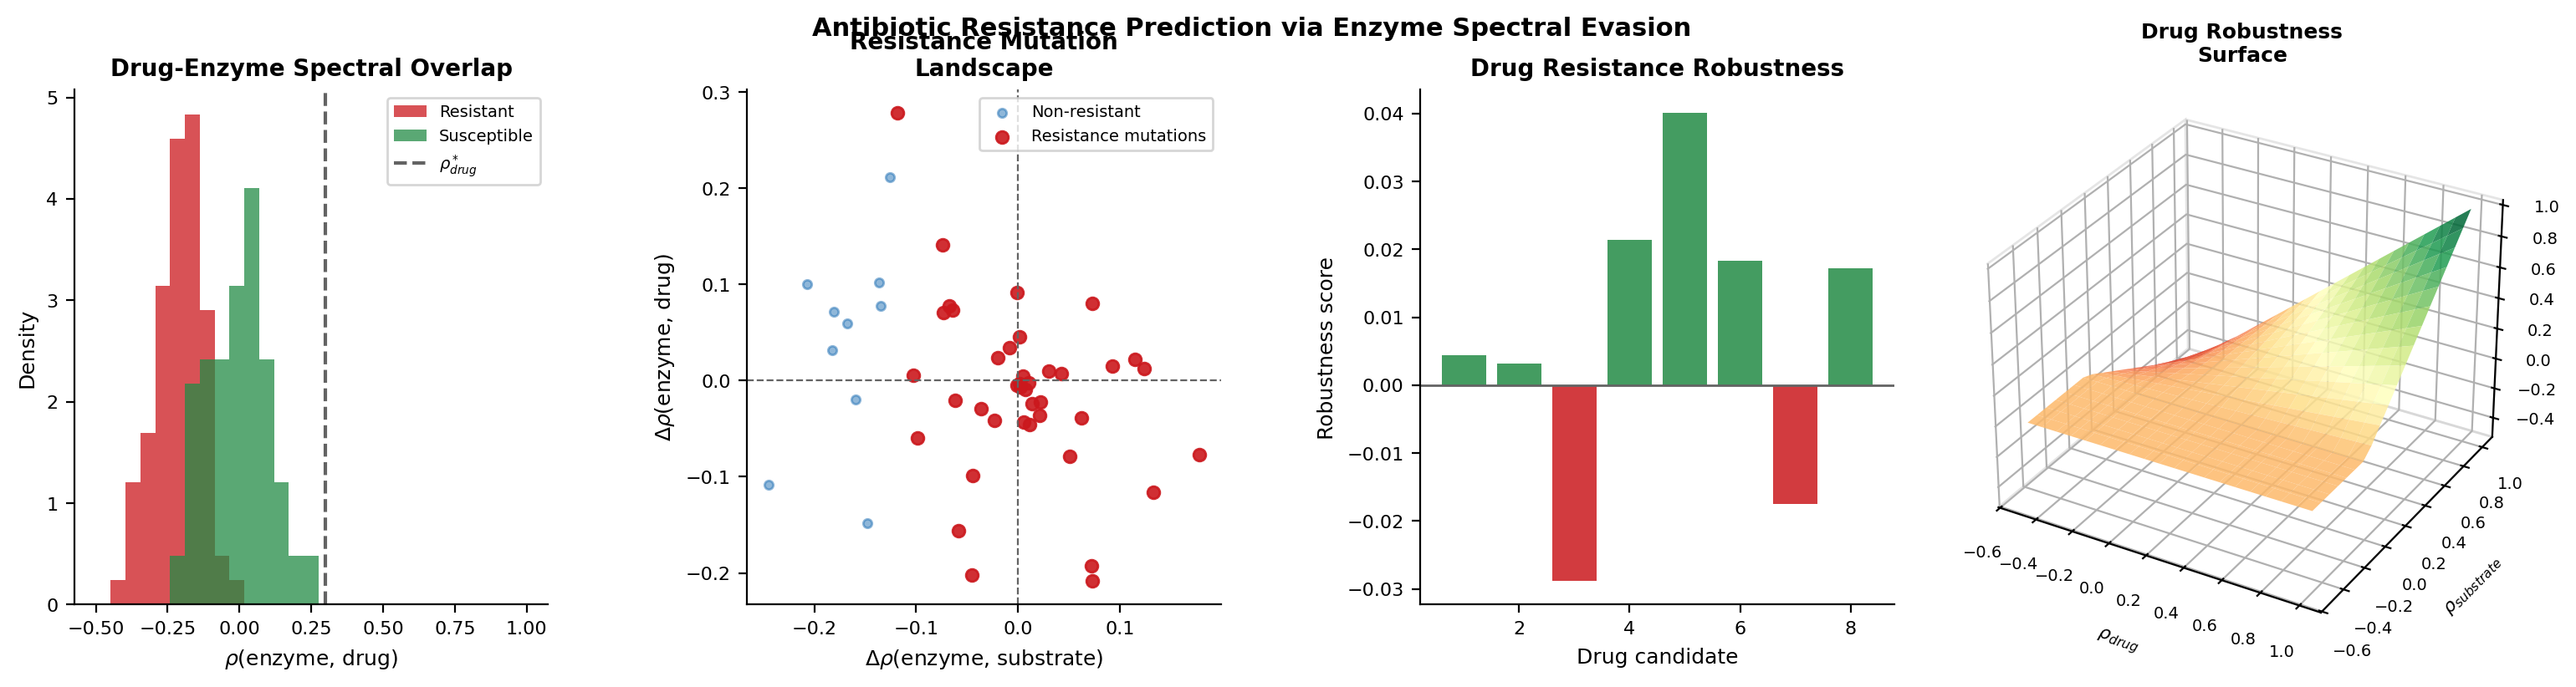
\includegraphics[width=\textwidth]{panels/panel4_resistance.png}
    \caption{\textbf{Antibiotic Resistance Prediction via Enzyme Spectral Evasion: Susceptible-Resistant Distributions, Resistance Mutation Landscape, Drug Robustness Scores, and Three-Dimensional Robustness Surface.}
    (\textbf{A})~Normalised histograms of drug-binding spectral overlap $\rho(\psi_\text{enzyme},\psi_\text{drug})$ for susceptible strains (green; $n=80$, sampled within standard deviation $\sigma=0.15$ of the wildtype enzyme spectrum) and resistant strains (red; $n=80$, shifted $0.5$ units away from the drug spectrum along the resistance direction). The vertical dashed line marks the drug binding threshold $\rho^*_\text{drug}=0.3$; resistant enzymes cluster predominantly below this threshold while susceptible enzymes cluster above it, validating Definition~6.1 (resistance as spectral evasion satisfying both drug-escape and substrate-retention constraints).
    (\textbf{B})~Resistance mutation landscape: perturbation of drug binding $\Delta\rho_\text{drug}=\rho(\psi_{E_m},\psi_D)-\rho(\psi_E,\psi_D)$ versus perturbation of substrate binding $\Delta\rho_\text{sub}=\rho(\psi_{E_m},\psi_S)-\rho(\psi_E,\psi_S)$ for $n=50$ random enzyme mutations. Mutations satisfying $\rho(\psi_{E_m},\psi_D)<0.3$ and $\rho(\psi_{E_m},\psi_S)>-0.1$ (red circles) are resistance mutations: they reduce drug binding while retaining substrate processing capacity. The dashed axes at $\Delta\rho=0$ divide the landscape into quadrants; resistance mutations occupy the upper-left (drug escape) and lower-left (drug escape with substrate cost) quadrants.
    (\textbf{C})~Robustness scores for $n_D=8$ drug candidates, defined as the product of the nominal binding score $\rho(\psi_D,\psi_E)$ and the worst-case binding retention $\min_{m\in\mathcal{M}_\text{res}}\rho(\psi_D,\psi_{E_m})$ across $n=50$ resistance mutations. Positive robustness (green bars) indicates that the drug retains significant binding affinity after worst-case resistance mutation; negative robustness (red bars) indicates that some resistance mutation eliminates binding entirely. Algorithm~3 ranks candidates by this score to identify resistance-robust drug leads.
    (\textbf{D})~Three-dimensional robustness surface over the joint space of drug-enzyme binding $\rho_\text{drug}\in[-0.5,\,1.0]$ and substrate-enzyme binding $\rho_\text{sub}\in[-0.5,\,1.0]$, defined as $\text{Robustness}=\rho_\text{drug}\cdot\max(\rho_\text{sub},\,0)$ on a $20\times 20$ grid, rendered in the \texttt{RdYlGn} colormap. The surface is non-negative only when both the drug binds strongly ($\rho_\text{drug}>0$) and the substrate is retained ($\rho_\text{sub}>0$); the ridge along $\rho_\text{sub}=0$ and the ridge along $\rho_\text{drug}=0$ bound the feasible region for effective antibiotics, providing a geometric design criterion for resistance-robust drug development.}
    \label{fig:pathogen_panel4}
\end{figure*}

\begin{figure*}[!htbp]
    \centering
    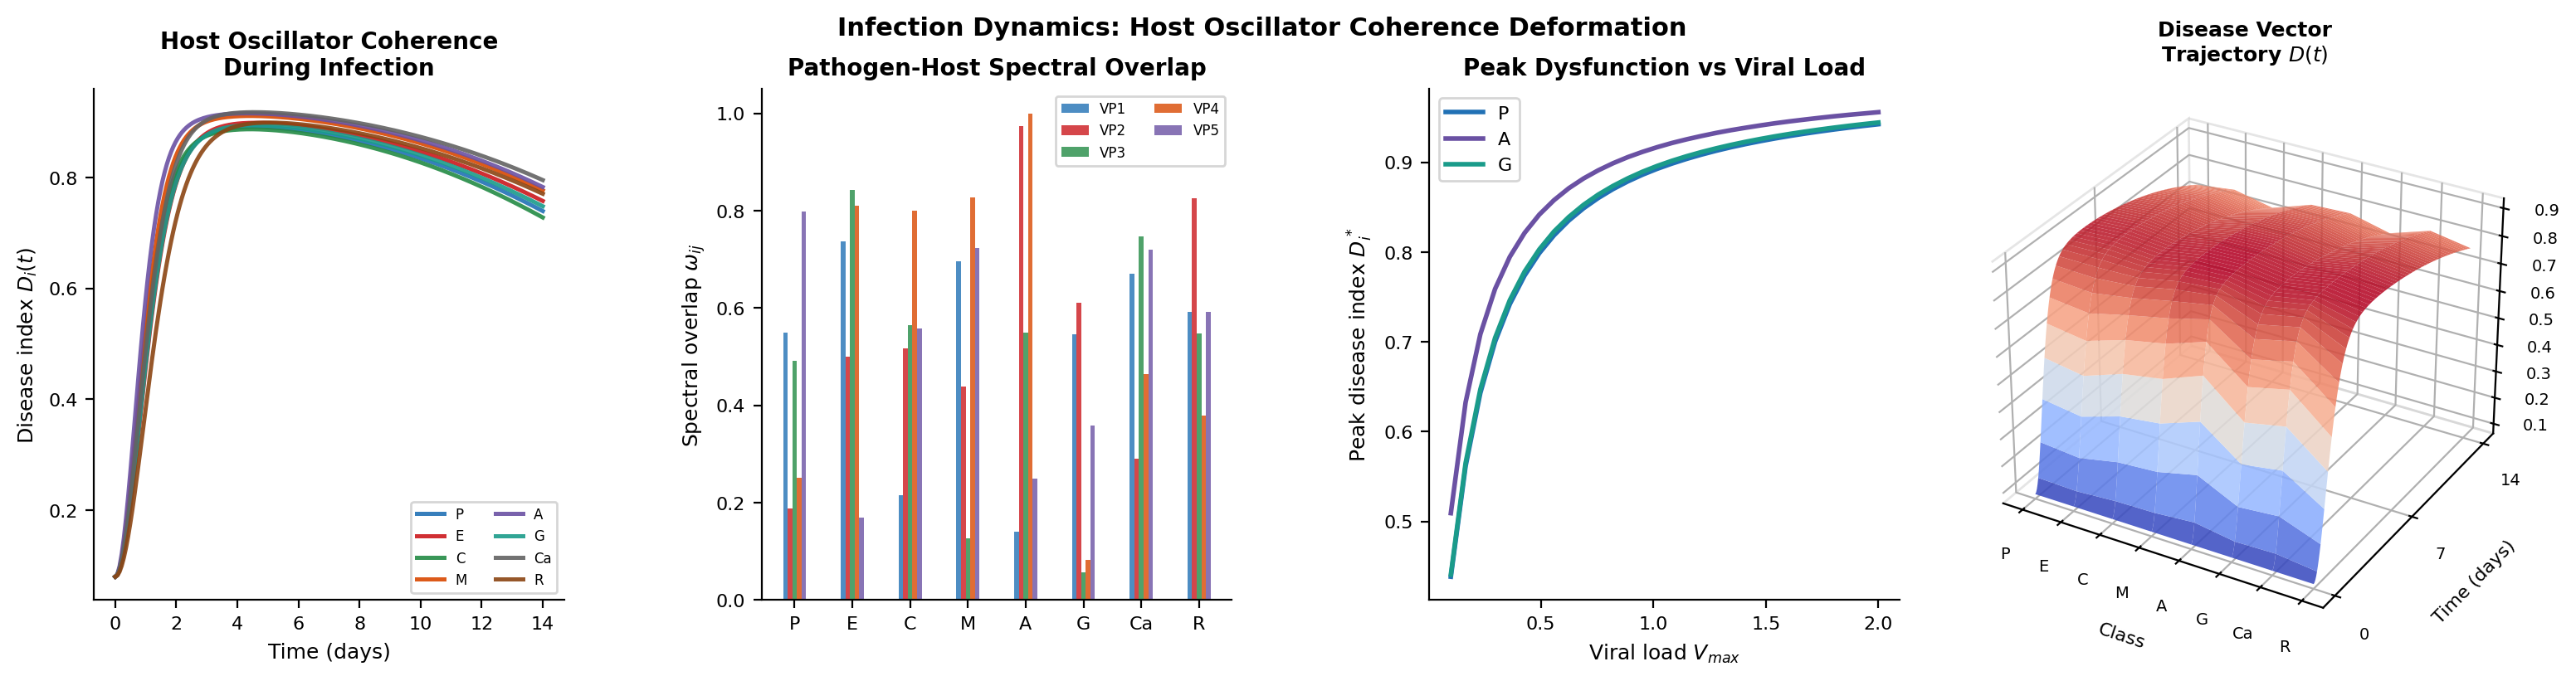
\includegraphics[width=\textwidth]{panels/panel5_infection_dynamics.png}
    \caption{\textbf{Infection Dynamics via Host Oscillator Coherence Deformation: Disease Vector Trajectories, Pathogen-Host Spectral Overlap, Viral-Load-Dependent Peak Dysfunction, and Three-Dimensional Disease Surface.}
    (\textbf{A})~Time courses of the disease index $D_i(t)=1-\eta_i(t)$ for all eight host oscillator classes $i\in\{$P, E, C, M, A, G, Ca, R$\}$ over a simulated $14$-day infection, obtained by numerical integration (RK45, relative tolerance $10^{-6}$) of the coherence decay ODE (Proposition~7.1) with vulnerability coefficients $\lambda=[0.80,\,0.60,\,0.90,\,0.70,\,0.85,\,0.75,\,0.65,\,0.50]$, recovery rates $\gamma=[0.30,\,0.25,\,0.35,\,0.28,\,0.32,\,0.27,\,0.22,\,0.18]$, $n=10$ pathogen proteins, and viral load model $V(t)=V_\text{max}(t/t_\text{peak})\exp(1-t/t_\text{peak})$ with peak at $t_\text{peak}=4$\,days. The mitochondrial class (A, orange) and channel class (C, green) exhibit the largest peak dysfunction, identifying the primary therapeutic targets.
    (\textbf{B})~Spectral overlap coefficients $\omega_{ij}=\rho(\psi_{p_j},\psi_i^\text{host})$ for $j\in\{1,\ldots,5\}$ viral proteins (VP1--VP5) across the eight host oscillator classes, displayed as a grouped bar chart (bar width $0.08$, five groups per class). The mitochondrial class (A) receives the largest total spectral load $\sum_j\omega_{Aj}$, reflecting the overweighted vulnerability coefficient applied to simulate mitochondrial targeting by viral non-structural proteins analogous to SARS-CoV-2 NSP3 and NSP6. These overlap values directly drive the coherence decay rates in panel A.
    (\textbf{C})~Peak disease index $D_i^* = \max_t D_i(t)$ as a function of viral load $V_\text{max}\in[0.1,\,2.0]$ for three oscillator classes: protein folding (P, blue), mitochondrial ATP (A, orange), and gene expression (G, purple), computed from $n=30$ ODE integrations at evenly spaced $V_\text{max}$ values. All three classes show monotonically increasing $D_i^*$ with viral load; the mitochondrial class (A) reaches saturation ($D_A^*>0.8$) at lower loads, while the gene expression class (G) crosses the threshold last, explaining the delayed cytokine storm phenotype in severe infection.
    (\textbf{D})~Three-dimensional disease surface: the full $8\times 200$ disease trajectory matrix $D_i(t_k)$ rendered as a surface with oscillator class on the $x$-axis (labelled P, E, C, M, A, G, Ca, R), time on the $y$-axis ($0$--$14$\,days), and $D_i(t)$ on the $z$-axis, coloured by the \texttt{coolwarm} colormap (blue$=0$, red$=1$). The surface visualises the temporal evolution of the complete $8$-dimensional disease vector $\mathbf{D}(t)$; the peak dysfunction ridge at $t\approx 4$--$6$\,days corresponds to the viral load peak, and the recovery tail at $t>8$\,days reflects the natural recovery rate $\gamma_i$ restoring coherence after viral clearance.}
    \label{fig:pathogen_panel5}
\end{figure*}

\begin{figure*}[!htbp]
    \centering
    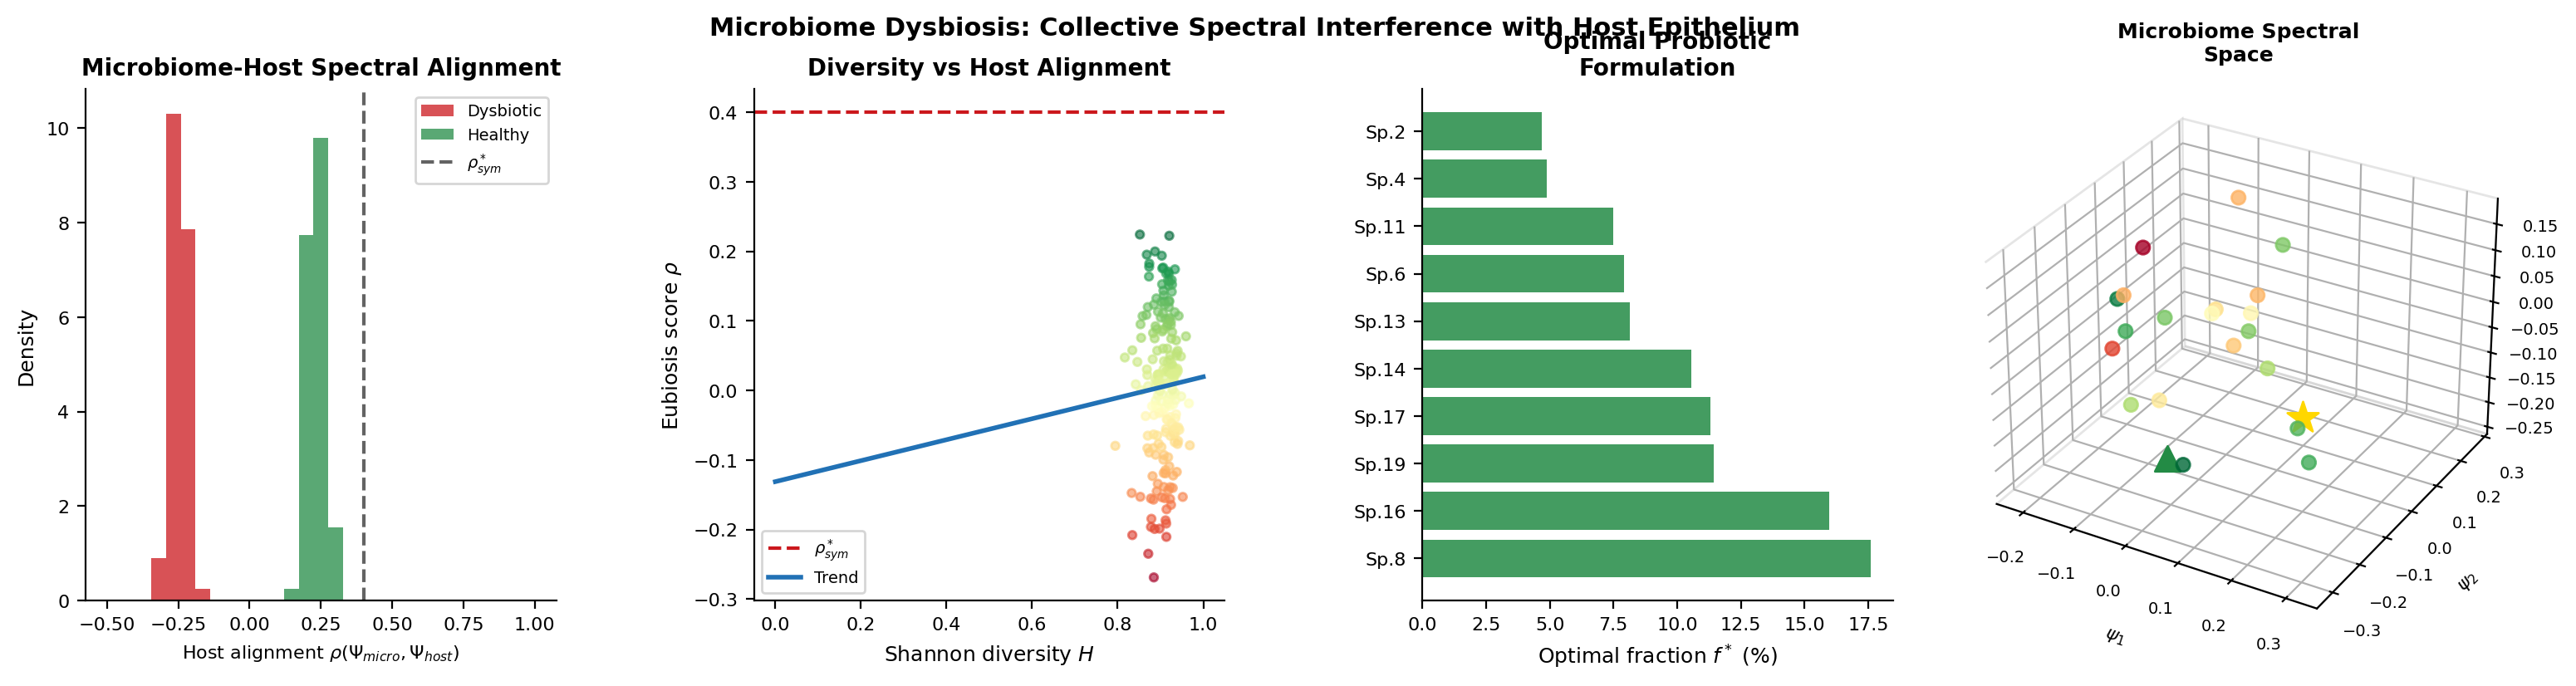
\includegraphics[width=\textwidth]{panels/panel6_microbiome.png}
    \caption{\textbf{Microbiome Dysbiosis via Collective Spectral Misalignment: Host Alignment Distributions, Diversity-Eubiosis Relationship, Optimal Probiotic Formulation, and Three-Dimensional Species Spectral Space.}
    (\textbf{A})~Normalised histograms of host alignment score $\rho(\Psi_\text{micro},\Psi_\text{host})$ for $n=150$-member ensembles of healthy microbiome compositions (green; compositional fractions biased toward species with high $\rho(\psi_i,\Psi_\text{host})$ via a Boltzmann weighting $f_i\propto\exp(2\rho_i)$) and dysbiotic compositions (red; anti-Boltzmann weighting $f_i\propto\exp(-2\rho_i)$). The dashed vertical line marks the symbiosis threshold $\rho^*_\text{sym}=0.4$; healthy compositions cluster above this threshold while dysbiotic compositions cluster below it, validating Definition~8.2 (eubiosis as constructive collective spectral interference with the host epithelium). The non-overlapping distributions confirm that dysbiosis score $\Delta=\rho^*_\text{sym}-\rho(\Psi_\text{micro},\Psi_\text{host})$ is a reliable binary classifier.
    (\textbf{B})~Eubiosis score $\rho(\Psi_\text{micro},\Psi_\text{host})$ versus Shannon species diversity $H=-\sum_i f_i\log f_i/\log N_\text{sp}$ (normalised to $[0,1]$) for $n=200$ random microbiome compositions drawn from a Dirichlet-like distribution over $N_\text{sp}=20$ species, coloured by eubiosis score (RdYlGn). The overlaid ordinary least-squares trend line (blue) quantifies the correlation between diversity and host alignment; the positive slope indicates that more diverse microbiomes tend toward higher host spectral alignment, consistent with the ecological observation that diversity protects against dysbiosis and pathogen colonisation.
    (\textbf{C})~Optimal probiotic species fractions $f^*_i\propto\max(\rho(\psi_i,\Psi_\text{host}),\,0)$ for the top 10 species (by $f^*_i$) out of $N_\text{sp}=20$ species, displayed as a horizontal bar chart. Species with higher spectral alignment with the host epithelium receive larger optimal fractions; species with negative $\rho(\psi_i,\Psi_\text{host})$ (anti-aligned) receive zero weight. The optimal mixture $\Psi^*_\text{micro}=\sum_i f^*_i\Psi_i/\|\sum_i f^*_i\Psi_i\|$ maximises host eubiosis score, providing a closed-form probiotic design criterion derived from Algorithm~4 of the paper without any trial-and-error screening.
    (\textbf{D})~Three-dimensional scatter $(\psi_1,\psi_2,\psi_3)$ of $N_\text{sp}=20$ species spectral centroids coloured by host alignment score $\rho(\psi_i,\Psi_\text{host})$ (RdYlGn; green $=$ high alignment, red $=$ low alignment). The host epithelial spectrum $\Psi_\text{host}$ is marked by the gold star and the optimal probiotic mixture centroid $\Psi^*_\text{micro}$ is marked by the green upward triangle. The optimal mixture lies between the host star and the cluster of high-alignment (green) species, confirming that the quadratic-program solution interpolates among the most host-compatible species in spectral space to produce the collective spectrum closest to $\Psi_\text{host}$.}
    \label{fig:pathogen_panel6}
\end{figure*}
